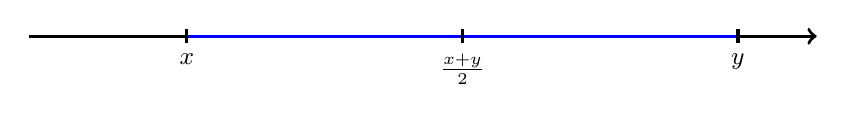
\begin{tikzpicture}
  \coordinate (A) at (-5,0);
  \coordinate (B) at (5,0);
  
  \draw [very thick,\lt->] (A) -- (B); 
  \draw [very thick,blue] (-3,0) -- (4,0);
  \draw [very thick] (-3,2.5pt) -- +(0,-5pt) node [anchor=north, font=\small] {$x$};
  \draw [very thick] (4,2.5pt) -- +(0,-5pt) node [anchor=north, font=\small] {$y$};
  \draw [very thick] (.5,2.5pt) -- +(0,-5pt) node [anchor=north, font=\small] {$\frac{x + y}{2}$};
\end{tikzpicture}
